%!TEX root = draft.tex
%\newcommand{\seqPQ}{\mathsf{SeqPQ}}

\section{Compositionality of Distributed Linearizability}
\label{sec:compositionality of distributed linearizability}




\subsection{Definition of Compositionality}
\label{subsec:definition of compositionality}

The following is the definition of distributed linearizability for multi-object histories.

\begin{definition}[Distributed Linearizability for Multi-object Histories]
\label{definition:distributed linearizability for multi-object histories}
A multi-object history $h$ is distributed linearizabile, if there exists a sequence $\mathit{lin}$, called linearization of $h$, such that

\begin{enumerate}[(i)]
\item The elements of $\mathit{lin}$ is generated from the operations of $h$: each operation $o = (m(a) \Rightarrow b,i,\mathit{obj})$ is transformed into $(m(a) \Rightarrow b,i,S)$ with $S$ set of identifiers of operations of visible to $o$ via $h.\mathit{vis}$.
\item $\mathit{lin}$ is consistent with $h. \mathit{vis}$.
\item For each object $\mathit{obj}$, $h \uparrow_{\mathit{obj}}$ is distributed linearizable, and $\mathit{lin} \uparrow_{ \mathit{obj} }$ is a linearization of $h \uparrow_{\mathit{obj}}$.
\end{enumerate}

A set $H$ of multi-object histories are distributed linearizable w.r.t deterministic sequential specifications, if each of its history is.
\end{definition}

The following is the definition of compositional histories.

\begin{definition}[Compositionality]
\label{definition:compositionality}
A multi-object history $h$ is called compositional, if: $h \uparrow_{\mathit{obj}}$ is distributed linearizable for each object $\mathit{obj}$, if and only if, $h$ is distributed linearizable.
\end{definition}

It is easy to see that, a multi-object history $h$ being distributed linearizable implies that the projection of $h$ into each object is distributed linearizable. When proving compositionality, we only need to consider the opposite direction.




\subsection{T0-Linearizability and T1-Linearizability}
\label{subsec:t0-linearizability and t1-linearizability}

T0-linearizability is a sub-class of distributed linearizability.

\begin{definition}[t0-linearizability]
\label{definition:t0-ilnearizability}
A single-object history $h$ is t0-linearizable w.r.t a sequential specification $\mathit{spec}$, if for each distributed linearizable history $h=(\mathit{Op},\mathit{ro},\mathit{vis})$, a sequence $\mathit{lin}$ shown below is a linearization of $h$ w.r.t $\mathit{spec}$:

\begin{itemize}
\setlength{\itemsep}{0.5pt}
\item[-] Each element $(\ell,i,\mathit{vis}^{-1}(i))$ of $\mathit{lin}$ is generated from an operation $(\ell,i,\_,\mathit{ts})$ of $h$.

\item[-] $\mathit{lin}$ is consistent with $\mathit{vis}$.
\end{itemize}
\end{definition} 

To prove t0-linearizability, we introduce the notion of , A specification $\mathit{spec}$ is called t0-specification, if given a history $h$ that is distributed linearizable w.r.t $\mathit{spec}$, then any sequence that is consistent with visibility relation is a linearization of $h$.



The following lemma states some example of t0-linearizability. Their proof can be found in Appendix \ref{subsec:appendix definitions and proofs in subsection subsec t0-linearizability and t1-linearizability}

\begin{lemma}
\label{lemma:several t0-specifications}
The or-set implementation is t0-linearizable w.r.t $\mathit{OR}$-$\mathit{set}_s$, and the counter implementation is t0-linearizable w.r.t $\mathit{counter}_s$.
\end{lemma}





For a history where time-stamp is used for conflict resolution, such as RGA and last-write-win register (LWW-register), we can assume that each operation also gives the information of time-stamp. Or we can say, we can implicitly assume that each operation is of the form $o = (\ell,i,\mathit{obj},\mathit{ts})$, where $\mathit{ts}$ is the ``time-stamp'' of this operation: %A set of method is selected and called special method.

\begin{itemize}
\setlength{\itemsep}{0.5pt}
\item[-] If $o$ generates a new unique time-stamp, then $\mathit{ts}$ is this new time-stamp.

\item[-] If $o$ does not generate new time-stamp, then $\mathit{ts}$ is the maximum of time-stamp among operations visible to $o$.

\item[-] Moreover, we require that given operations $o_1$ and $o_2$, if $(o_1,o_2) \in \mathit{vis}$, then the time-stamp of $o_1$ is less or equal than that of $o_2$.
\end{itemize}


\begin{definition}[t1-specification]
\label{definition:t1-specification}
A sequential specification $\mathit{spec}$ is a t1-specification, if for each distributed linearizable history $h=(\mathit{Op},\mathit{ro},\mathit{vis})$, a sequence $\mathit{lin}$ shown below is a linearization of $h$ w.r.t $\mathit{spec}$:

\begin{itemize}
\setlength{\itemsep}{0.5pt}
\item[-] Each element $(\ell,i,\mathit{vis}^{-1}(i))$ of $\mathit{lin}$ is generated from an operation $(\ell,i,\_,\mathit{ts})$ of $h$.

\item[-] $\mathit{lin}$ is consistent with $\mathit{vis}$.

\item[-] If the time-stamp of $o_1$ is less than that of $o_2$, then $o_1$ is before $o_2$ in $\mathit{lin}$. Or we could say, $\mathit{lin}$ is consistent with time-stamp.
\end{itemize}
\end{definition}

The following lemma shows several t1-specifications. Its proof can be found in Appendix \ref{subsec:proof in subsection subsec t0 specification and t1 specification}

\begin{lemma}
\label{lemma:several t1-specifications}
$\mathit{reg}_s$ and $\mathit{list}_s^{\mathit{af}}$ are t1-specification.
\end{lemma}

\begin{table}
  \centering
  \begin{tabular}[t]{l|l}
    T0 & Counter, Set, \\
    T1 & RGA,
  \end{tabular}
\end{table}




\subsection{Composing Several t0-Specifications}
\label{lemma:several t0-specifications can be composed}

The following lemma states that a history of several objects of t0 specifications is compositional. Its proof can be found in Appendix \ref{subsec:appendix proofs of lemma several t0-specifications can be composed}.

\begin{restatable}{lemma}{composingTZero}
\label{lemma:several t0-specifications can be composed}
Given a multi-object history $h$, if each of its object uses a t0-specification, then, $h$ is compositional.
\end{restatable}




\subsection{Composing Several t0-Specifications with One T1-specification}
\label{lemma:composing several t0-specification with one t1-specification}

Composing several t0-specifications with one t1-specification does not hold in general. \figurename~\ref{fig:a failed example of composing a multi-value register with a last-write-win register} is a history $h$ that is a failed example of composing a multi-value register with a last-write-win register, where the operations of LWW register are boxed. Here we assume that $\mathit{ts}_1<\mathit{ts}_2$. Since multi-value register is t0-specification and LWW register is t1-specification, we can see that the projection of $h$ into operations of multi-value register is distributed linearization and the only possible linearization is $\mathit{write}(a) \cdot \mathit{write}(b)$, and the projection of $h$ into operations of LWW register is distributed linearization and the only possible linearization is $\mathit{write}(c) \cdot \mathit{write}(d)$. However, $h$ is not distributed linearizable, since there is a a cycle.

\begin{figure}[t]
  \centering
  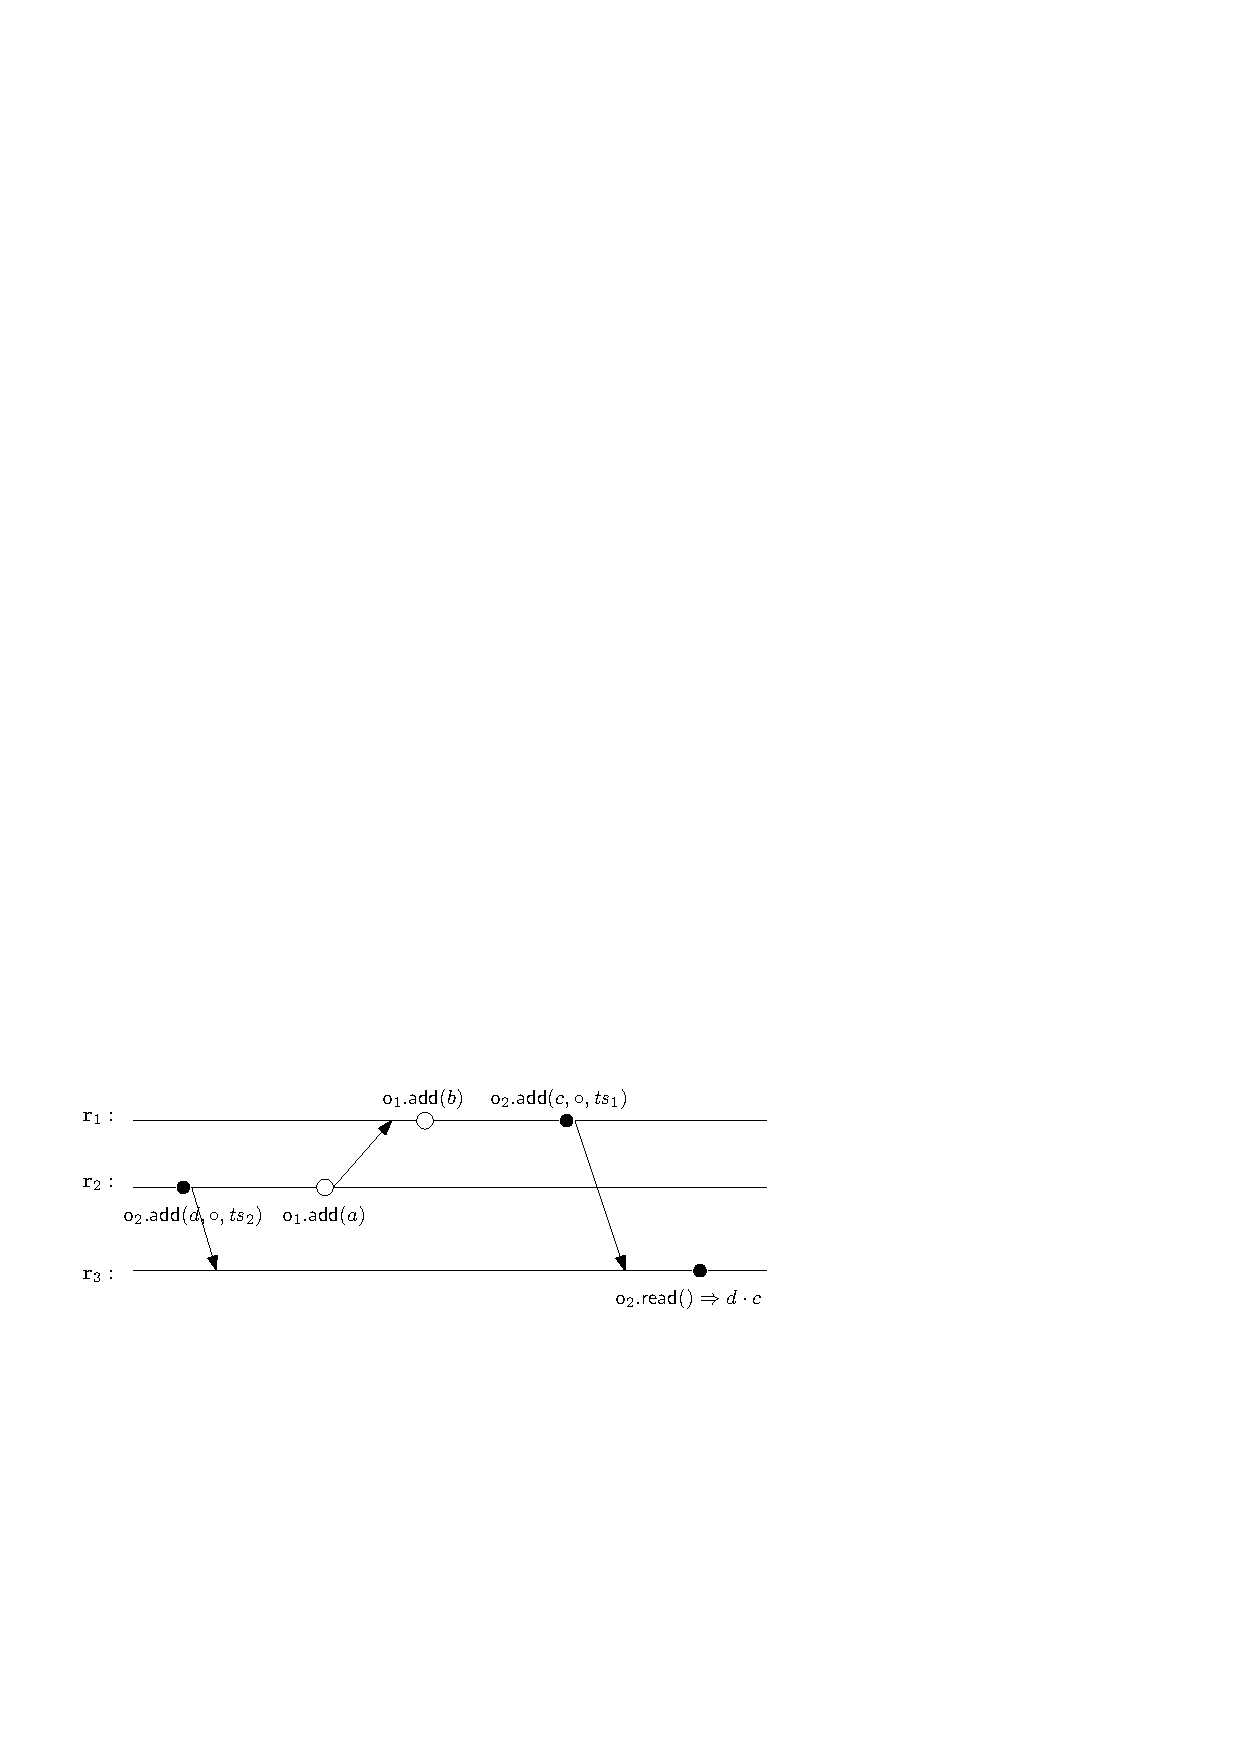
\includegraphics[width=0.6 \textwidth]{figures/MVReg-LWWReg-Nocd.pdf}
\vspace{-10pt}
  \caption{A failed example of composing a multi-value register with a last-write-win register (boxed operations), where $\mathit{ts}_1 < \mathit{ts}_2$.}
  \label{fig:a failed example of composing a multi-value register with a last-write-win register}
\end{figure}

The following lemma states that for a multi-object history, if its object use several t0-specifications and one t1-specification, and its visibility relation is transitive, then, $h$ is compositional. Its proof can be found in Appendix \ref{subsec:appendix proofs of lemma several t0-specifications and one t1-specification can be composed}.

\begin{restatable}{lemma}{composingTZeroAndOneTOne}
\label{lemma:several t0-specifications and one t1-specification can be composed}
Given a multi-object $h$, if its object use several t0-specifications and one t1-specification, and its visibility relation is transitive, then, $h$ is compositional.
\end{restatable}




\subsection{Composing Several t0-Specifications with Several T1-specification}
\label{lemma:composing several t0-specification with several t1-specification}

Composing several t0-specifications with several t1-specification does not hold in general. \figurename~\ref{fig:a failed example of composing two last-write-win registers} is a history $h$ that is a failed example of composing two last-write-win registers, where the operations of one LWW register are boxed, and the operations of the other LWW registers are not boxed. Here we assume that $\mathit{ts}_1 < \mathit{ts}_2 < \mathit{ts}_3$, and $\mathit{ts}'_1 < \mathit{ts}'_2$. Since LWW register is t1-specification, we can see that the projection of $h$ into operations of one LWW register is distributed linearization and the only possible linearization is $\mathit{write}(a,\mathit{ts}'_1) \cdot \mathit{write}(b,\mathit{ts}'_2)$, and the projection of $h$ into operations of the other LWW register is distributed linearization and the only possible linearization is $\mathit{write}(c,\mathit{ts}_1) \cdot \mathit{write}(d,\mathit{ts}_2) \cdot \mathit{write}(e,\mathit{ts}_3)$. However, $h$ is not distributed linearizable, since there is a a cycle.

\begin{figure}[t]
  \centering
  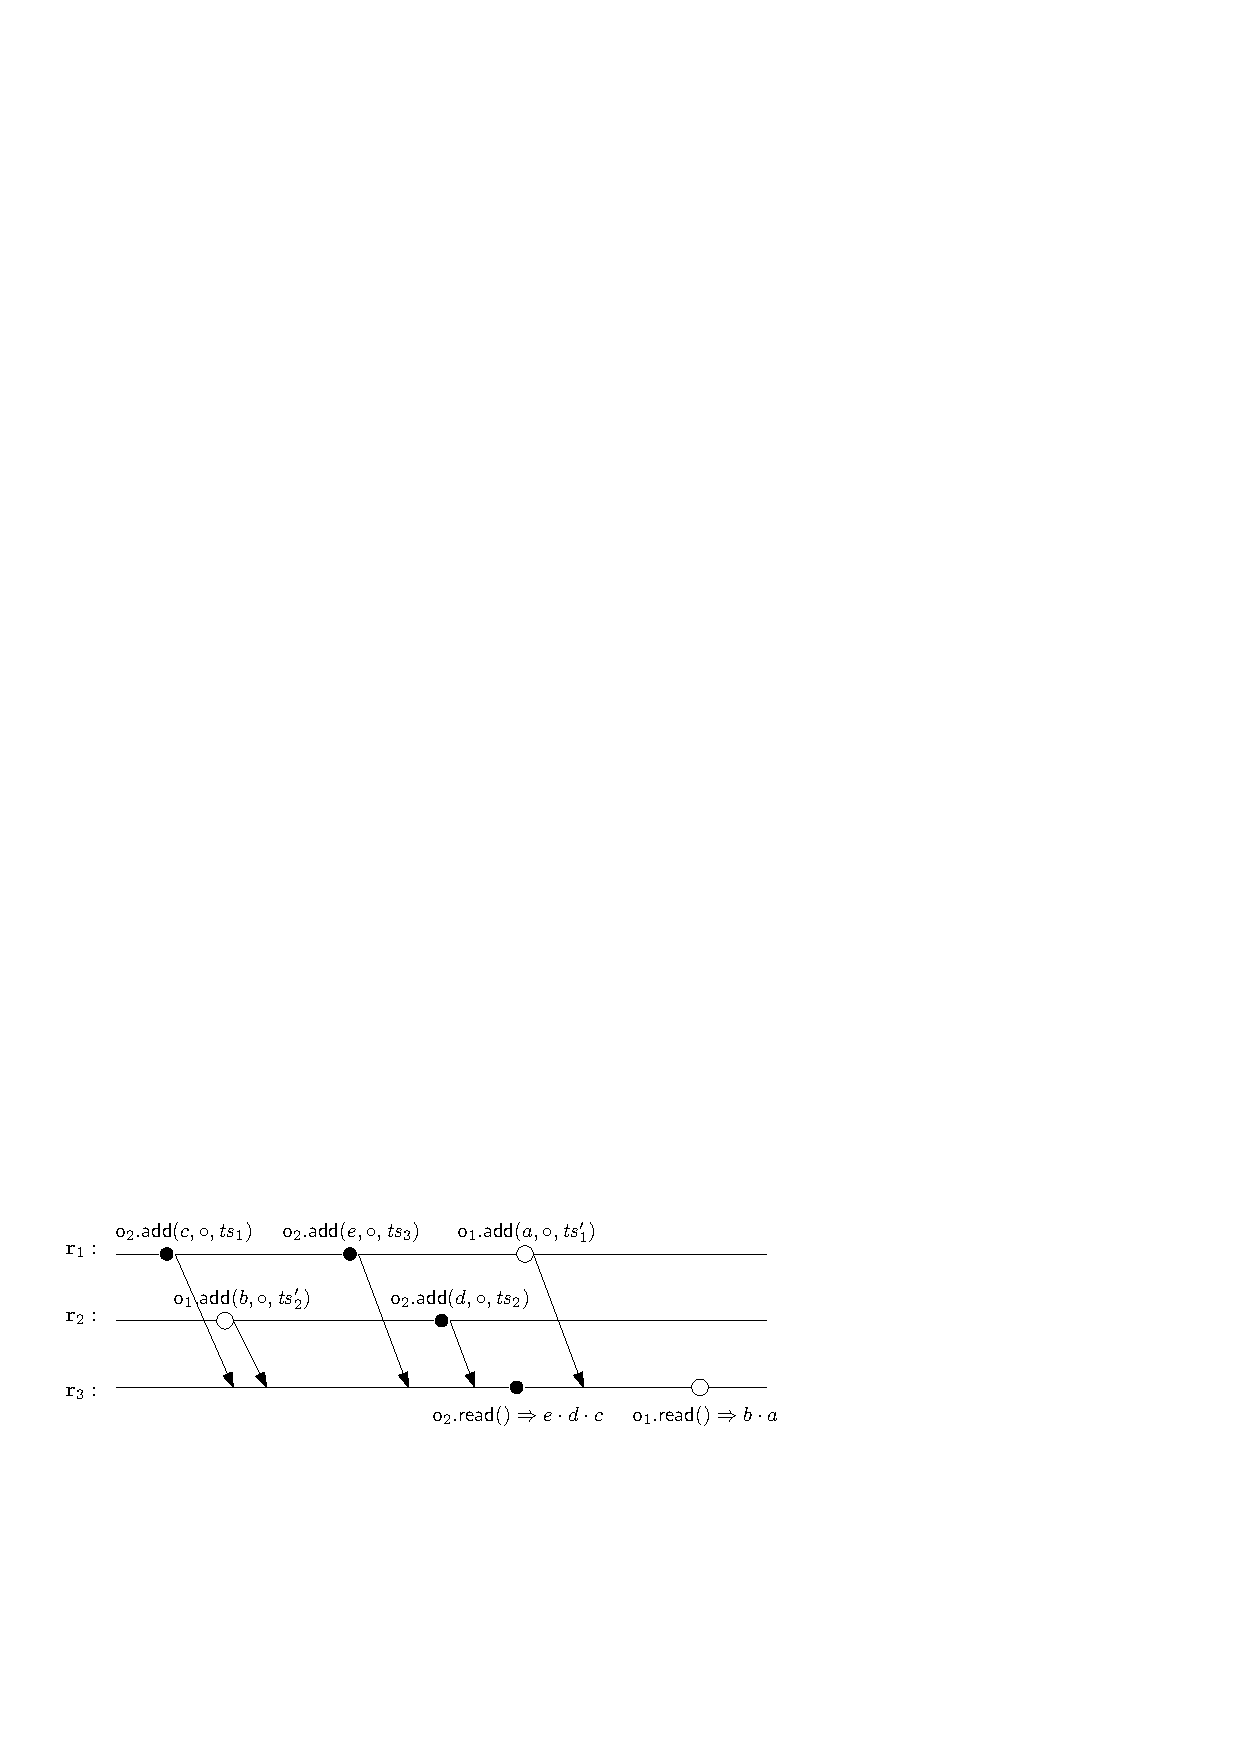
\includegraphics[width=0.7 \textwidth]{figures/LWWReg-LWWReg-NoSTS.pdf}
\vspace{-10pt}
  \caption{A failed example of composing two last-write-win registers (one object is boxed, the other is not), where $\mathit{ts}_1 < \mathit{ts}_2 < \mathit{ts}_3$, and $\mathit{ts}'_1 < \mathit{ts}'_2$.}
  \label{fig:a failed example of composing two last-write-win registers}
\end{figure}


A history $h$ satisfies causal-time-stamp, if: Given operation $o_1,\ldots,o_{\mathit{2k+2}}$ of $h$ that are of objects of t1-specification, if

\begin{itemize}
\setlength{\itemsep}{0.5pt}
\item[-] $(o_2,o_3)$ are of a same object, $\ldots$, $(o_{\mathit{2k}},o_{\mathit{2k+1}})$ are of a same object, $(o_{\mathit{2k+2}},o_1)$ are of a same object,

\item[-] $\mathit{ts}(o_2) < \mathit{ts}(o_2)$, $\ldots$, and $\mathit{ts}(o_{\mathit{2k}}) < \mathit{ts}(o_{\mathit{2k+1}})$,

\item[-] $(o_1,o_2), \ldots, (o_{\mathit{ek+1}},o_{\mathit{2k+2}}) \in \mathit{vis}$.
\end{itemize}

Then, we have $\mathit{ts}(o_1) < \mathit{ts}(o_{\mathit{2k+1}})$.

The following lemma states that for a multi-object history, if its object use several t0-specifications and several t1-specification, and it satisfies causal-time-stamp and its visibility relation is transitive, then, $h$ is compositional. Its proof can be found in Appendix \ref{subsec:appendix proofs of lemma several t0-specifications and several t1-specification can be composed}.

\begin{restatable}{lemma}{composingTZeroAndTOne}
\label{lemma:several t0-specifications and several t1-specification can be composed}
Given a multi-object $h$, if its object use several t0-specifications and several t1-specification, and it satisfies causal-time-stamp and its visibility relation is transitive, then, $h$ is compositional.
\end{restatable}





\subsection{Semantics of Multi Objects}
\label{subsec:semantics of multi objects}

When there is multiple objects, we say $(o_1,o_2) \in \mathit{vis}$, if either $(o_1,o_2) \in \mathit{ro}$, or $o_1$ is delivered to the replica of $o_2$ before $o_2$ happens. We consider CTDT implementation of t1-specifications use the time-stamp of Lamport's time-stamp: Each time-stamp is a tuple $(c,r)$ of a counter value $c \in \mathbb{N}$ and a replica identifier $r \in \mathbb{R}$; $(c_1,r_1) < (c_2,r_2)$, if $c_1 < c_2 \vee (c_1 = c_2 \wedge r_1 < r_2)$. To ensure compositionality of multiple objects, the following conditions needs to be satisfied:

\begin{itemize}
\setlength{\itemsep}{0.5pt}
\item[-] Cross-object-causal-delivery (COCD): We extend the notion of causal-delivery into multiple objects. Given two update operations $o_1$ and $o_2$, and assume $o_1$ is visible to $o_2$. Then, for each replica, once it receives $o_2$, it must be the case that $o_1$ has been previously received.

\item[-] Shared-time-stamp (STS): the objects of t1-specifications shares a counter $\mathit{sCtr}$. Each message carries a value of $\mathit{sCtr}$, and when generating new message, the value of $\mathit{sCtr}$ is also considered.
\end{itemize}



Based on shared-time-stamp,



Formally, given a set $\mathit{Objs}$ of objects, its semantics is defined as $\llbracket \mathit{Objs} \rrbracket_{\mathit{op}} = (\mathit{Config},\mathit{config}_0,\Sigma',\rightarrow)$ as in \figurename~\ref{fig:the semantics of multiple operation-based CRDT object}.


\begin{figure}[ht]
$\mathit{RState} = \mathit{Objs} \times \mathbb{R} \rightarrow \Sigma$

$\mathit{TState} = \mathbb{MID} \times \mathbb{MSG} \times \mathbb{R} \times \mathit{Objs}$

$\mathit{MsgHB} \subseteq \mathbb{MID} \times \mathbb{MID}$

$\mathit{MsgDel} \subseteq \mathbb{MID} \times \mathbb{R}$

$\mathit{Config} = \mathit{RState} \times \mathit{TState} \times \mathit{MsgHB} \times \mathit{MsgDel}$, $\mathit{config}_0 \in \mathit{Config}$.

$\Sigma' = \mathit{do}(\mathit{Objs} \times \mathbb{M} \times \mathbb{D} \times \mathbb{D} \times \mathbb{R} \times \mathbb{MID}) \cup \mathit{do}(\mathit{Objs} \times \mathbb{M} \times \mathbb{D} \times \mathbb{D} \times \mathbb{R}) \cup \mathit{receive}(\mathit{Objs} \times \mathbb{MID} \times \mathbb{R})$

\begin{itemize}
\setlength{\itemsep}{0.5pt}
\item[] $\begin{array}{l c}
   \bigfrac{
   \begin{array}{c}
     R(x,r) = \sigma, (x,r).\mathit{do}(\sigma,m,a) = (\sigma',b,\mathit{msg}), \mathit{msg} \neq \emptyset, \mathit{unique}(\mathit{mid}), \\
     S_1 = \{ (\mathit{mid}',\mathit{mid}) \vert (\mathit{mid'},r) \in \mathit{MsgDel} \}, S_2 = \{ (\mathit{mid}',\mathit{mid}) \vert \mathit{mid}' \in T, \mathit{mid}' \ is \ of \ replica \ r \}
   \end{array}}
     {(R,T,\mathit{msgHB},\mathit{MsgDel}) {\xrightarrow{\mathit{do}(x,m,a,b,r,\mathit{mid})}} (R[(x,r):\sigma'], T \cup \{ (\mathit{mid},\mathit{msg},r,x) \}, (\mathit{MsgHB} \cup S_1 \cup S_2)^*,\mathit{MsgDel})}
\end{array}$

\item[] $\begin{array}{l c}
   \bigfrac{
   \begin{array}{c}
     R(x,r) = \sigma, (x,r).\mathit{do}(\sigma,m,a) = (\sigma',b,\emptyset)
   \end{array}}
     {(R,T,\mathit{msgHB},\mathit{MsgDel}) {\xrightarrow{\mathit{do}(x,m,a,b,r)}} (R[(x,r):\sigma'], T \cup \{ (\mathit{mid},\mathit{msg},r) \}, \mathit{MsgHB},\mathit{MsgDel})}
\end{array}$

\item[-] $\begin{array}{l c}
   \bigfrac{
   \begin{array}{c}
      R(x,r) = \sigma, (x,r).\mathit{receive}(\sigma,\mathit{msg}) = \sigma', (\mathit{mid},\mathit{msg},r',x) \in T, r \neq r', \\
      (\mathit{mid},r) \notin \mathit{MsgDel}, \mathit{mid} \ is \ minimal \ w.r.t \ \mathit{MsgHB} \ among \ \{ \mathit{mid}' \vert (\mathit{mid}',r) \notin \mathit{MsgDel} \}
   \end{array}}
     {(R,T,\mathit{msgHB},\mathit{MsgDel}) {\xrightarrow{\mathit{receive}(x,\mathit{mid},r)}} (R,T,\mathit{MsgHB},\mathit{MsgDel} \cup \{ (\mathit{mid},r) \} )}
\end{array}$
\end{itemize}
\caption{The definition of semantics of $\llbracket \mathit{Objs} \rrbracket_{\mathit{op}}$}
\label{fig:the semantics of multiple operation-based CRDT object}
\end{figure}




$R$ is now a function from object and replica identifier to local state. Message and action also record its object. $\mathit{MsgHB}$ and $\mathit{MsgDel}$ now record the relation between messages of multiple objects. In each transition rule of \figurename~\ref{fig:the semantics of multiple operation-based CRDT object}, we deal with each object according to its CRDT implementations. Similarly, a sequence $l$ of actions is an execution of $\llbracket \mathit{Objs} \rrbracket_{\mathit{op}} = (\mathit{Config},\mathit{config}_0,\Sigma',\rightarrow)$, if there exists $(R,T,\mathit{MsgHB},\mathit{MsgDel}) \in \mathit{Config}$, such that $\mathit{config}_0 {\xrightarrow{ l }} (R,T,\mathit{MsgHB},\mathit{MsgDel})$. The semantics of $\mathit{Objs}$ is defined as the set of executions of $\llbracket \mathit{Objs} \rrbracket_{\mathit{op}}$.





A configuration $(R,T,\mathit{MsgHB},\mathit{MsgDel})$ is a snapshot of distributed system. $R$ gives the local state of each replica, and $T$ gives the set of messages that has been generated. Let $\mathbb{MID}$ be the set of message identifiers of message content. A message is a tuple $(\mathit{mid},\mathit{msg},r)$, where $\mathit{mid} \in \mathbb{MID}$ is the identifier, $\mathit{msg} \in \mathbb{MSG}$ is the message content, and $r$ is the original replica of message. $\mathit{MsgHB}$ is used to record the happen-before relation between messages: two messages $(\mathit{mid}_1,\mathit{mid}_2) \in \mathit{MsgHB}$ represents that the operation of $\mathit{mid}_1$ happens before the operation of $\mathit{mid}_2$. $\mathit{MsgDel}$ is used to record the message delivery relation between messages: $(\mathit{mid},r) \in \mathit{MsgDel}$ represents that message $\mathit{mid}_1$ has already been delivered to replica $r$. $\mathit{MsgHB}$ and $\mathit{MsgDel}$ are used to ensure message delivery requirements. $\mathit{config}_0$ is the initial configuration, which maps each replica into the initial local state, has no message, and with a empty happen-before relation and a empty message delivery relation.


Each element of $\Sigma'$ is called an action. $\rightarrow \in \mathit{Config} \times \Sigma' \times \mathit{Config}$ is the transition relation and describes a single step of distributed systems. The first rule in \figurename~\ref{fig:the semantics of a operation-based CRDT object} describes replica $r$ performs a update operation $m(a) \Rightarrow b$ and generates a message with message content $\mathit{msg}$. Here $\mathit{unique}$ is a function that ensures $\mathit{mid}$ be a fresh message identifier. We insert message identifier $\mathit{mid}$ into the happen-before relation and keeps the happen-before relation be transitive. The second rule describes replica $r$ performs a query operation $m(a) \Rightarrow b$ and thus does not generate message. Since no message is generated, the $\mathit{MsgHB}$ and $\mathit{MsgDel}$ tuples remain the same. The third rule describes delivery of a message to a replica $r$ other than its origin replica $r'$. By $(\mathit{mid},r) \notin \mathit{MsgDel}$, we ensure that $\mathit{mid}$ has not been previously delivered to replica $r$, and thus, each message be delivered to each replica at most once. By $\mathit{mid}$ being minimal w.r.t $\mathit{MsgHB}$ among $\{ \mathit{mid}' \vert (\mathit{mid}',r) \notin \mathit{MsgDel} \}$, we always choose a minimal element w.r.t $\mathit{MsgHB}$ among operations not been delivered to a replica, and thus, ensures causal-delivery.



\subsection{Proving in Multi-Objects Semantics}
\label{subsec:proving in multi-object semantics}


The formation of CRDT in this semantics is changed as follows,

The CRDT proved distributed linearizable are still distributed linearizable in this new semantics.


%%% Local Variables:
%%% mode: latex
%%% TeX-master: "draft"
%%% End:
